\section{Hadronic Calorimeter}
\label{sec:hcal}
The hadronic calorimeter (HCAL) is designed to measure the energy of hadrons while providing good shower containment and hermicity.
The HCAL surrounds the ECAL and is inside the solenoid, with the exception of the hadronic outer (HO) detector which is placed just outside the solenoid.
The purpose of the HO is to catch any hadronic showers which are not fully contained within the bulk of the HCAL.
A schematic of the HCAL subsystem layout is shown in Figure \ref{fig:hcallayout}.
The HCAL is a sampling calorimeter in that it utilizes scintillating plastic tiles with embedded wavelength-shifting fibers (WLS), interspersed between brass absorber plates.
A hadron traveling through the HCAL will interact with the brass absorber producing a hadronic shower which produces photons as the particles in the shower pass through the scintillating tiles.
The photons captured in the tiles are then carried via the WLS to the hybrid photodiode based readout system.
%As the HCAL is a sampling calorimeter the radial profile of the hadronic shower can be measured by using each of the tiles separately giving an additional parameter to the measurement of the deposited energy.
\begin{figure}[htpb]
\begin{center}
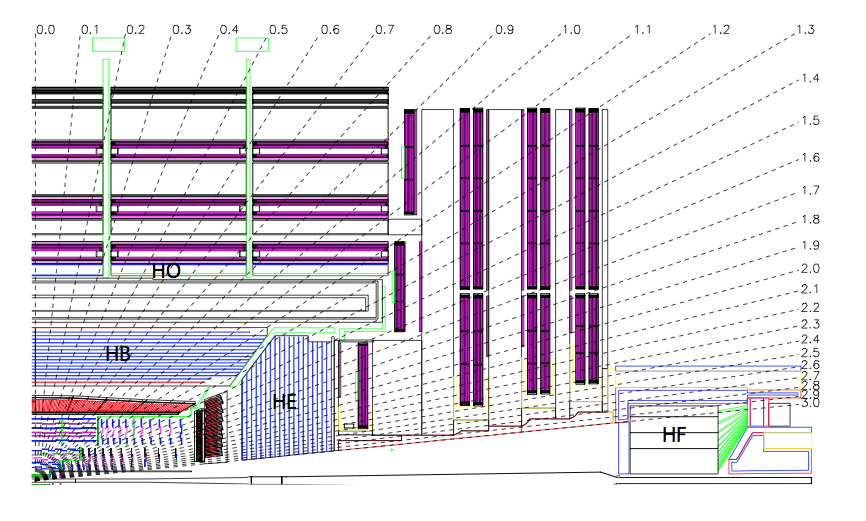
\includegraphics[width=0.9\textwidth]{plots/hcallayout.png}
\caption{Schematic of the CMS hadronic calorimeter subsystem\cite{CMS_DETECTOR}.}
\label{fig:hcallayout}
\end{center}
\end{figure}

A forward calorimeter (HF) is used in addition to the HCAL barrel, endcaps, and HO. 
The HF spans the region from $\pm3.0$ to $\pm5.0$ in $\eta$, and is designed to measure the hadronic energy deposited in the congested high $\eta$ region.
Not only does the HF provide the ability to measure hadronic energy in the high $\eta$ regions, but also provides a method to measure the luminosity delivered to the CMS detector.
The HF is a Cherenkov detector with quartz fibers, running parallel to the beam line,  installed into grooves situated inside a steel absorber.
Hadronic showers that originate in the steel absorber will contain neutral and charged particles that will produce Cherenkov light if their energy is above a certain threshold.
The Cherenkov light is then measured to reconstruct the energy deposited in the calorimeter.
The quartz fibers used have two lengths where one length is shorter than the other, providing a means of separating electrons and photons from hadrons.
This is possible as showers produced from incident electrons and photons will deposit their energy very quickly and not travel as far as showers produced from incident hadrons.

The jet $E_{T}$ resolution as a function of transverse energy is shown in Figure \ref{fig:jetres}. The $E_{T}$ resolution is better than $20\%$ for jets with $E_{T} > 50$ GeV, and drops to $10\%$ for jets with $E_{T} > 300$ GeV.
\begin{figure}[htpb]
\begin{center}
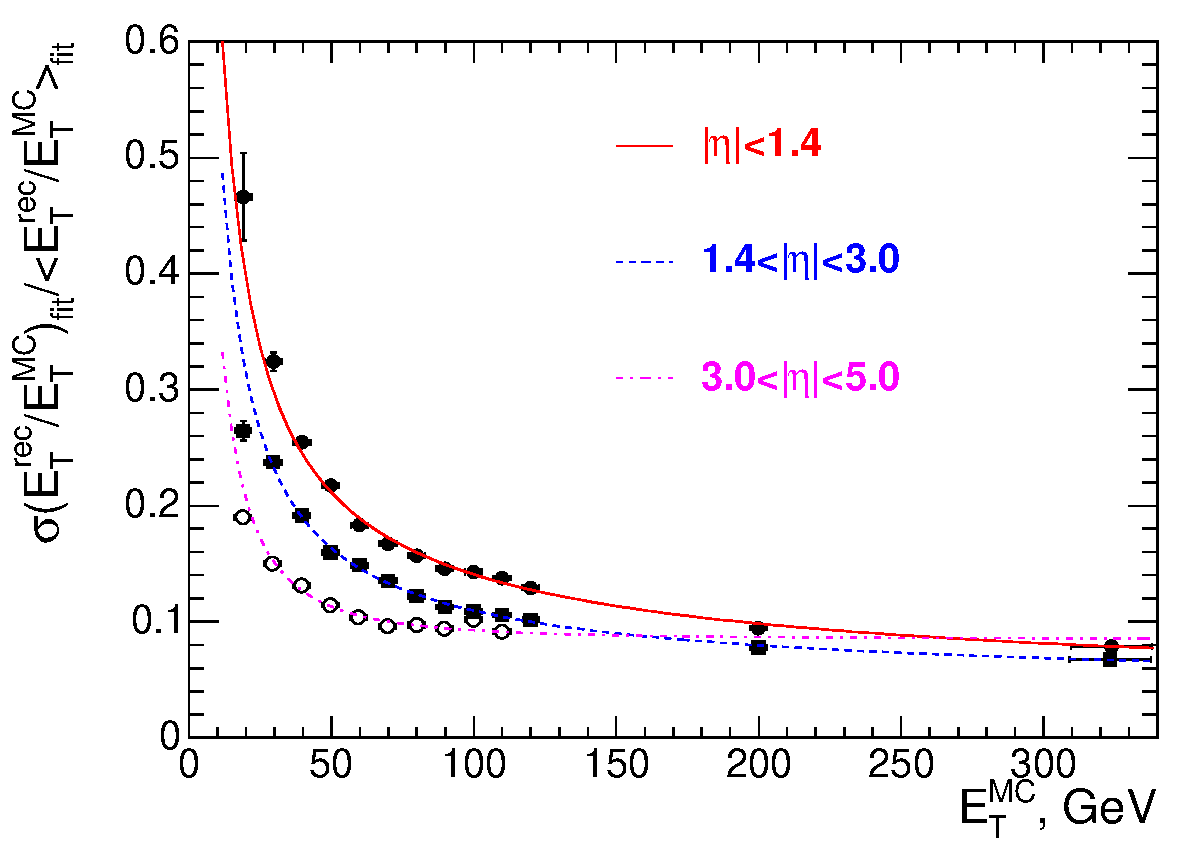
\includegraphics[width=0.85\textwidth]{plots/jetres.pdf}
\caption{Jet energy resolution for the HCAL in the barrel, endcap and forward regions\cite{CMS_DETECTOR}.}
\label{fig:jetres}
\end{center}
\end{figure}
